
The intrusion kill chain introduced by Lockheed-Martin\cite{Hutchins_Cloppert_Amin} describes the steps an actor takes in attacking a target system. The specifics of each step vary by situation and objective, but the process provides a foundation on which to build and compare models.


\begin{figure}[ht]
\centering
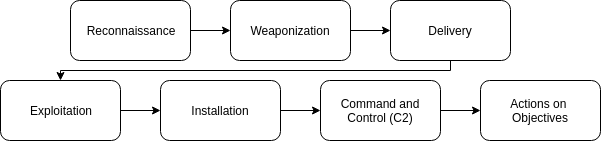
\includegraphics[width=.8\linewidth]{resource/img/ch_background/intrusion_kill_chain.png}
\caption{LM Intrusion Kill Chain\cite{Hutchins_Cloppert_Amin}}
\label{fig:background:kill_chain}
\end{figure} 

Attacks against networks can be motivated by many factors, but the effects generally fall into one of a handful of categories\cite{Chakrabarti_Govindarasu_2002}. Our threat model assumes an attacker originating outside the core network boundary intends to target a device within the core network, permitting the attacker to view or alter a victim's traffic. In other words, identifying the potential for \textit{eavesdropping} and \textit{tampering} is the focus of this research, and we address the limitations of modeling network \textit{disruption} later in this section. Table \ref{tab:threats} lists some common attack patterns against Layer 2 and 3 networks. In general these attacks are used to redirect a target's traffic through an asset controlled by the attacker, or to escalate the attacker's privileges on systems that interact with the target. We briefly review these attack classes here in order to present our Datalog models in the following sections.



% Vulns
\begin{table}[ht]
\centering
\captionsetup{justification=centering}
\caption{Potential Threats}
\resizebox{.4\textwidth}{!}{%
% \begin{small}
\begin{tabular}{@{}lll@{}}
\toprule
% Layer 2 & Layer 3  &  \\ \midrule
VLAN Hopping & ACL Bypass \\
STP Injection & BGP Hijacking \\
ARP Cache Poisoning & Route Table Poisoning &  \\
MAC Flooding & SYN Flooding &  \\
CAM Overflow & Packet Crafting &  \\
MAC/DHCP Spoofing & IP Spoofing &  \\
%MPLS Attachment Point &  IPSec AH/IKE \\ 
\bottomrule
\end{tabular}%
% \end{small}
}
\label{tab:threats}
\end{table}

We frame our threat discussion within Layers 2 and 3 of the OSI 7-layer model here for clarity, but don't limit our analysis to only these vectors. These attacks often aren't the goal of an attacker, but rather enable the attacker to reach their goal through the effects of the compromise. For example, traffic eavesdropping may reveal credentials for a privileged account on some other system the attacker has interest in. 



\begin{figure}[ht]
  \centering
% \noindent\begin{minipage}[t]{0.98\linewidth}
\begin{bytefield}[bitwidth=1em]{39}
% \begin{bytefield}{39}
\bitbox[]{35}{$\overbrace{\hspace{34em}}^{\text{\normalsize L1 Eth Packet (72--1530B)}}$} & \bitbox[]{4}{} \\
\bitbox[]{6}{} &
\bitbox[]{29}{$\overbrace{\hspace{28em}}^{\text{\normalsize L2 Eth Frame (64--1522B)}}$} \\
\bitbox[]{21}{} &
\bitbox[]{9}{$\overbrace{\hspace{10em}}^{\text{\normalsize L3 Packet (46--1500B)}}$}  & \bitbox[]{9}{}  \\
    \begin{rightwordgroup}{802.3 field}
       \bitbox{3}{Pre} &  \bitbox{3}{SFD}  & 
        \bitbox{4}{src}  & \bitbox{4}{dst} & 
        \bitbox{4}{VLAN}  & \bitbox{3}{len} &
        \bitbox{10}{Payload}  & \bitbox{4}{CRC}
         & \bitbox{4}{IPG} 
    \end{rightwordgroup} \\
    \begin{rightwordgroup}{Bytes in field}
    \bitbox[]{3}{7} &  \bitbox[]{3}{1}  & 
        \bitbox[]{4}{6}  & \bitbox[]{4}{6} & 
        \bitbox[]{4}{4}  & \bitbox[]{3}{2} &
        \bitbox[]{10}{46--1500}  & \bitbox[]{4}{4}
         & \bitbox[]{4}{12} 
     \end{rightwordgroup}
    % \\ \bitbox[]{8}{$\underbracebrace{\hspace{11em}}_{\text{\normalsize Header}}$}
\end{bytefield}
% \end{minipage}
 \caption{802.3 Ethernet Packet Layout}
  \label{fig:bits_802_3}
\end{figure}


\textbf{Layer 2 Attacks:} 
\begin{itemize}
\item CAM Overflow: Hardware switches use \textit{Content Addressable Memory} tables to map devices to the port they are connected to. When frames enter the ingress switch port, a CAM table entry is created for the source MAC address and port if it doesn't exist. The destination MAC address is found in the CAM table and the frame is forwarded out the associated port. If no destination entry is found the frame is flooded out all ports, and the CAM table is updated with the port the destination MAC responds from. The CAM is implemented in hardware and has a fixed size buffer. If an attacker can exhaust the CAM buffer by generating enough unique source addressed frames to fill the table, the switch will flood any traffic without an entry to every switch port, allowing an attacker to eavesdrop traffic from any connected device on the native VLAN. 
\item  ARP Spoofing: The \textit{Address Resolution Protocol}\cite{Plummer} maps Layer 2 MAC addresses to Layer 3 IP addresses. To find a MAC address for a given IP target, an ARP request is broadcast to all members of the local subnet. The owner of the IP address then sends an ARP reply containing their MAC address. RFC 826 allows for unsolicited ARP replies, meaning that any system on the local subnet can announce that they own any IP or MAC address without the address first being requested by a peer. An attacker announcing ownership of an address will receive all traffic destined for that address. 
\item VLAN Hopping: \textit{Virtual LANs} allow the creation of multiple logically separate broadcast networks over the same Layer 2 switch. The 802.1Q VLAN field in Figure \ref{fig:bits_802_3} accepts a 12 bit VLAN tag to differentiate 4094 possible VLANs, with later extensions to the standard allowing over 16 million tags. Since VLANs are isolated broadcast domains, communication between VLAN nodes must be routed over a Layer 3 protocol. VLAN tags are written to Ethernet frames by the ingress switch either statically based on attachment port, or dynamically based on some policy like the source MAC address. The primary VLAN connection types are \textit{Access} links which connect a host to a switch using a single tag, \textit{Trunk} links which interconnect switches and carry tags for all VLANs, and the default \textit{Native} VLAN which allows untagged traffic and is typically used for management. The link type is configured for each switch port manually over the management interface, dynamically using a protocol like DTP (dynamic trunking protocol), or it falls back to the default which is vendor and model specific. If a switch port the attacker is connected to is not explicitly configured as an Access port, the attacker can present themselves as a peer switching device (known as \textit{Switch Spoofing}) and craft the DTP packets to negotiate a Trunk port, resulting in access to traffic on any managed VLAN. Another VLAN bypass can be accomplished if the attacker is allowed to write arbitrary data to the VLAN tag field, which is permitted by members of the Native VLAN. In this scenario, an attacker can send traffic to a target on another VLAN by \textit{Double Tagging} messages. The outer VLAN tag is popped by the first receiving switch and then flooded out all of its Native VLAN ports. The inner tag is now read by the receiving switch and the message is sent to the victim. This is a blinded attack since no response will be returned from the malicious traffic.
% \item STP 
% \item DHCP
% \item MPLS
\end{itemize}

% \begin{figure*}
%   \centering
%   \begin{bytefield}{32}
%     \bitheader{31,24,23,16,15,8,7,0} \\
%     \bitbox{1}{\tiny{M\\E\\M}} & \bitbox{3}{SEL} & \bitbox{23}{} & \bitbox{4}{Mem\\Type} & \bitbox{4}{ID} \\    
%   \end{bytefield}
%   \caption{\label{fig:mwe_cmd}Cmd word}
% \end{figure*}


% \begin{figure}[ht]
%   \centering
% \begin{bytefield}[bitwidth=1em]{32}
%     \bitheader{0-31} \\
%     % \begin{rightwordgroup}{RTP \\  Header}
%         \bitbox{4}{V=6} & \bitbox{8}{Traffic Class} & \bitbox{20}{Flow Label} \\
%         \bitbox{16}{Payload Length}  & \bitbox{8}{Next Header} & \bitbox{8}{Hop Limit} \\
%     % \end{rightwordgroup} \\
%     \wordbox[tlr]{2}{128-bit Source Address} \\
%     \wordbox[tlr]{2}{128-bit Destination Address} \\
%     \wordbox[blr]{1}{$\cdots$} \\
% \end{bytefield}
%  \caption{IPv6 frame format rfc8200}
%   \label{fig:bits_ipv6}
% \end{figure}


% Layer 2 Attacks: 

% 



\begin{figure}[ht]
  \centering
  \begin{bytefield}{32}
    \bitheader{0,7-8,15-16,23-24,31} \\
    \begin{rightwordgroup}{transport \\ header}
      \bitbox{8}{protocol version} &
      \bitbox{8}{packet type} &
      \bitbox{8}{type modifier} &
      \bitbox{8}{client channel} \\
      \wordbox{1}{source connection identifier} \\
      \wordbox{1}{destination connection identifier} \\
      \wordbox{1}{message acceptance criteria} \\
      \wordbox{1}{heartbeat} \\
      \bitbox{16}{window} &
      \bitbox{16}{retention}
    \end{rightwordgroup} \\
  \begin{rightwordgroup}{data \\ fields}
    \wordbox[lrt]{1}{%
     {(data content and format dependent on packet type and modifier)}} \\
    \skippedwords \\
    \wordbox[lrb]{1}{} 
  \end{rightwordgroup}
  \end{bytefield}
  \caption{MTP packet format}
  \label{fig:bits_tcp}
\end{figure}

